
\section{Star-galaxy Separation Methodology}

We first briefly review the Bayesian star-galaxy separation method proposed in SIL2020 and then
apply it to single-band Rubin data, followed by its extension to multi-band case. Our principal
measured object property is the difference between PSF, \(m_{\mathrm{PSF}}\), and CModel, \(m_{\mathrm{CModel}}\),
magnitudes, \(\Delta m = m_{\mathrm{PSF}} - m_{\mathrm{CModel}}\). For unresolved sources, this \(\Delta m \)
is vanishing within noise, while for resolved objects \(\Delta m > 0\) (see Figure~\ref{fig:truth_morphology_color}).
A comparison and statistical discussion of this quantity and several other quantities proposed for
star-galaxy separation in the literature is available in SIL2020. 



\subsection{Bayesian Star-Galaxy Separation Method from SIL2020}

We first focus on the single-band case and then will extend our discussion to then multi-band case.
SIL2020 showed using realistic simulations that adopting a fixed pre-defined threshold for $\Delta
m$ in order to select resolved objects is not optimal. Not only that this threshold should depend
on magnitude due to variation of object populations, signal-to-noise ratio due to statistical noise,
and sky location due to varying count ratio of galaxies and stars, but for optimal combination of
information from different bands, or from other classification methods (e.g., based on colors),
observed $\Delta m$ distribution needs to be transformed into a proper probability density function. 

The subsample of objects with HST labels can be used to quantify $\Delta m$ distribution separately
for unresolved and resolved objects. However, such a ``training'' sample is currently available only
for a very small fraction of LSST footprint (less than 1\% of the area). Instead, we use the fact
that very large numbers of objects that remain even after binning in both sky location and magnitude
can robustly constrain two components of $\Delta m$ distribution even when such labels are not
available a priori. We only use the subsample of objects with HST labels to independently assess the
performance of our method. 


\subsection{Mixture Model for \(\Delta m\) vs. \(m_{\mathrm{CModel}}\) diagram \label{sec:mixmodel}} 

We assume that a sample is selected from a judiciously chosen sky region over which the variation
of stellar and galaxy population can be assumed statistically uniform. Over angular scales of
several degrees, stellar counts vary much more rapidly than galaxy counts (large galaxy clusters are
an exception but not important for subsequent discussion). Based on the analysis of state-of-the-art
Milky Way stellar population models by \cite{2025AJ....169..119P}, a sky region of several square
degrees, corresponding to Rubin tracts\footnote{In the Rubin Science Pipelines, tracts and patches
are the two levels of spatial subdivision used for coadded images and object catalogs. They are
designed to make processing and storage scalable while preserving continuity across the sky.
A tract is a relatively large region of the sky, approximately 1.75$^\circ$ x 1.75$^\circ$ (the exact
size depends on the sky map projection). that is processed as a unit. Tracts overlap slightly with
neighboring tracts to avoid edge effects. Each tract is subdivided into a regular grid of patches,
with each tract in DP2 containing 81 patches. The patch size is about 12 arcmin by 12 arcmin
(approximately, one CCD).}  is sufficiently small for this purpose (and consistent with our choice of
the COSMOS field for quantitative analysis). 
 
Given a ``tract'' catalog, and at a fixed CModel magnitude (see below for binning details), the
distribution of \(\Delta m\) in a given band (not explicitly marked for notational simplicity) is
modeled as a mixture of an unresolved (star) component and a resolved (galaxy) component, 
\begin{equation}
                                p(\dm \,|\, m) = w_U \, \funr (\dm) +  w_R \, \fres (\dm),
  \label{eq:mixpdf1}
\end{equation}
where $w_U + w_R = 1$, and $\funr$  and $\fres$  are properly normalized probability density
functions. With this decomposition, the probability that an object is unresolved is given by
Bayes' theorem as
\begin{equation}
        p_S(\dm) =p({\rm unr}\mid\dm)= \frac{w_U \funr(\dm)}  {w_U \funr (\dm) + w_R \fres (\dm)}.
  \label{eq:pSdm} 
\end{equation}
and the probability that it is resolved is $p_G = 1 - p_S$ (note that we use indices $S$ and
$unr$, or $G$ and $res$ interchangeably). 

The same model predicts the performance, the completeness and contamination for each class,
as function of a hard $\dm$ threshold. If $\dm<\dm_{\rm cut}$ is classified as unresolved,
\begin{equation}
                           {\rm Completeness}_S= \int_{-\infty}^{\dm_{\rm cut}}\funr (\dm) d\dm,
\end{equation}
and
\begin{equation}
                          {\rm Contamination}_S = \frac{w_U  \int_{-\infty}^{\dm_{\rm cut}}\funr (\dm) d\dm}
     {w_U \int_{-\infty}^{\dm_{\rm cut}}\funr (\dm) d\dm  + w_R \int_{-\infty}^{\dm_{\rm cut}}\fres (\dm) d\dm}.
\end{equation}
We test these predictions below using HST-based labels.
% However, one needs to be careful because HST labels are not perfect.
% There are HST stars that appear resolved in Rubin and have non-stellar colors (quasars, close
%  binary stars) and some HST galaxies are cannot be resolved using Rubin images obtained with
%  ground-based seeing.

Therefore, a good model for $p(\dm \,|\, m)$ (eq.~\ref{eq:mixpdf1}) is crucial. Informed by observed
$\dm$ distributions, we model the unresolved component, $\funr$ as a single Gaussian with mean
\(\mu_U\), width \(\sigma_U\) (and weight \(w_U\)).  The resolved component is modeled as a sum
of \(K\) log-normal distributions with weight \(w_{R,k}\), location
\(\mu_{R,k}\), scale \(\sigma_{R,k}\), and shape parameter \(\alpha_{R,k}\). The full
mixture probability density function is
\begin{equation}
  p(\Delta m \,|\, m) = w_U \, \mathcal{N}(\Delta m | \, \mu_U,\, \sigma_U)
    + \sum_{k=1}^{K} w_{R,k} \, \mathcal{LN}(\Delta m | \, \mu_{R,k},\, \sigma_{R,k},\, \alpha_{R,k}),
  \label{eq:mixture_pdf}
\end{equation}
where \(\mathcal{N}\) denotes the Gaussian and \(\mathcal{LN}\) the log-normal distribution,
and the weights are constrained to sum to unity: \(w_U = 1 - \sum_k w_{R,k}\) (functions
\(\mathcal{N}\) and \(\mathcal{LN}\) are properly normalized probability density functions).
The galaxy-to-star count ratio, which serves as Bayesian prior, is equal to
\begin{equation}
                   N_{GS} \equiv   {N_G \over N_S}  = {\sum_{k=1}^{K} w_{R,k}  \over  w_U}. 
\end{equation}
The expression given by eq.~\ref{eq:pSdm} can be recast as
\begin{equation}
              p_S(\dm) =   \frac{1}  {1 +  N_{GS}  \, BF},
  \label{eq:pSbf} 
\end{equation}
where Bayes factor is equal to
\begin{equation}
              BF = \frac{\fres} {\funr}. 
  \label{eq:bfdef} 
\end{equation}
With $N_{GS} \sim 30$ (see Figure~\ref{fig:star_galaxy_ratio_v8v9}), it is sufficient to have $BF \sim 0.033$
for $p_S$ to drop below 0.5 (because the sample is highly imbalanced).  This decomposition in terms of prior
and Bayes factor will be important later when combining multiple sources of classification information.  


\subsubsection{Fitting Details}

The fitting is performed independently in bins of CModel magnitude. At bright magnitudes
(\(m_{\mathrm{CModel}} < 22\)), where the resolved population is relatively simple, we use
\(K = 2\) resolved components in bins of width 1--3~mag spanning
\(15 < m_{\mathrm{CModel}} < 22\). At faint magnitudes (\(m_{\mathrm{CModel}} \geq 22\)),
where the galaxy morphology distribution is more complex, we use \(K = 3\) resolved components
in finer bins of width 0.5--1~mag spanning \(22 \leq m_{\mathrm{CModel}} < 27\). Within each
magnitude bin, \(\Delta m\) values in the range \((-0.5, 1.5)\) are binned into 300 bins
and normalized to unity. The mixture model is fit to these histograms using
bounded least-squares optimization with Poisson-like uncertainties
\(\sigma_i = \sqrt{N_i + 1} \,/\, (N \, \delta)\), where \(N_i\) is the count in bin \(i\),
\(N\) is the total number of sources in the magnitude slice, and \(\delta\) is the histogram
bin width.

This fitting procedure is carried out in three steps. In the first step, all mixture parameters
are fit independently in each magnitude bin. This free fit works well at bright magnitudes,
where unresolved and resolved sources are clearly separated in \(\Delta m\). However, at faint
magnitudes (\(m_{\mathrm{CModel}} \gtrsim 24\)), photometric noise broadens the unresolved
Gaussian until it becomes degenerate with the resolved components. The fitter can no longer
reliably distinguish the two populations, causing the unresolved Gaussian to absorb flux from
the galaxy distribution. This inflates the inferred star fraction at faint magnitudes.

To prevent this degeneracy, we impose smooth constraints on the unresolved component.
In the second step, the per-bin star parameters from step~1 are replaced with smooth
functions of magnitude: \(\mu_U\) is fixed to a single value (the median across all bins,
typically \(\approx 0\) in each band); \(\sigma_U(m)\) is fit with the photometric error model
from \citet{2007AJ....134.2236S} (their eq.~5),
\begin{equation}
  \sigma_U(m) = \sqrt{\sigma_0^2 + a^2 \cdot 10^{\,b\,(m - 25)}},
  \label{eq:sesar_sigma}
\end{equation}
where \(\sigma_0\), \(a\), and \(b\) are free parameters; and \(w_U(m)\) is modeled as a linear
fit to \(\log_{10}(w_U)\) versus magnitude, using only bins brighter than
\(m_{\mathrm{CModel}} = 24\) where the free fit is reliable. This smooth model is then
extrapolated to fainter magnitude bins. In the third step, with the unresolved component
(\(\mu_U\), \(\sigma_U\), \(w_U\)) fixed to the smooth curves from step~2, only the resolved
log-normal parameters are re-fit in each magnitude bin. The resolved weights are rescaled to
sum to \((1 - w_U)\) so that the total mixture remains a proper probability density.
The effectiveness of this constrained fitting procedure is demonstrated in
Figure~\ref{fig:star_galaxy_ratio_v8v9}, which compares the galaxy-to-star count ratio
\(\log_{10}(N_{\mathrm{gal}}/N_{\mathrm{star}})\) as a function of magnitude for models
with and without the smooth constraints. The unconstrained model exhibits a spurious turnover
at faint magnitudes, while the constrained model recovers the expected monotonically increasing
ratio in agreement with the COSMOS2020 external truth labels (note that in this sample at the faint
end galaxies outnumber stars by more than a factor of 30). 

\begin{figure*} 
  \centering
  
\includegraphics[width=\textwidth,height=0.62\textheight,keepaspectratio]{fig06_star_galaxy_ratio_vs_rmag_v8v9.png}
   \caption{Galaxy-to-star count ratio \(\log_{10}(N_{\mathrm{gal}}/N_{\mathrm{star}})\) vs.\
    r-band CModel magnitude. The unconstrained mixture model (marked V8, faded curves) exhibits a
    spurious turnover at \(m \gtrsim 24\) due to the unresolved Gaussian absorbing galaxy flux.
    The constrained model (marked V9, bold curves) recovers the expected monotonically increasing
    ratio, in good agreement with the COSMOS2020 truth labels (green dashed). Dotted lines show
    the Rubin \texttt{extendedness}-based classification for comparison (which also shows spurious
    turnover at the faint end.}
  \label{fig:star_galaxy_ratio_v8v9}
\end{figure*}

The model parameters are looked up by the CModel magnitude bin in which each source falls.
The quality of the fits is illustrated in Figure~\ref{fig:slice_fits}, which shows the
mixture model overlaid on the observed \(\Delta m\) histograms in each magnitude bin, and in
Figure~\ref{fig:model2d_residuals}, which shows the 2D data, model, and residual maps in the
\(\Delta m\) vs.\ \(m_{\mathrm{CModel}}\) plane.

\begin{figure*}
  \centering
  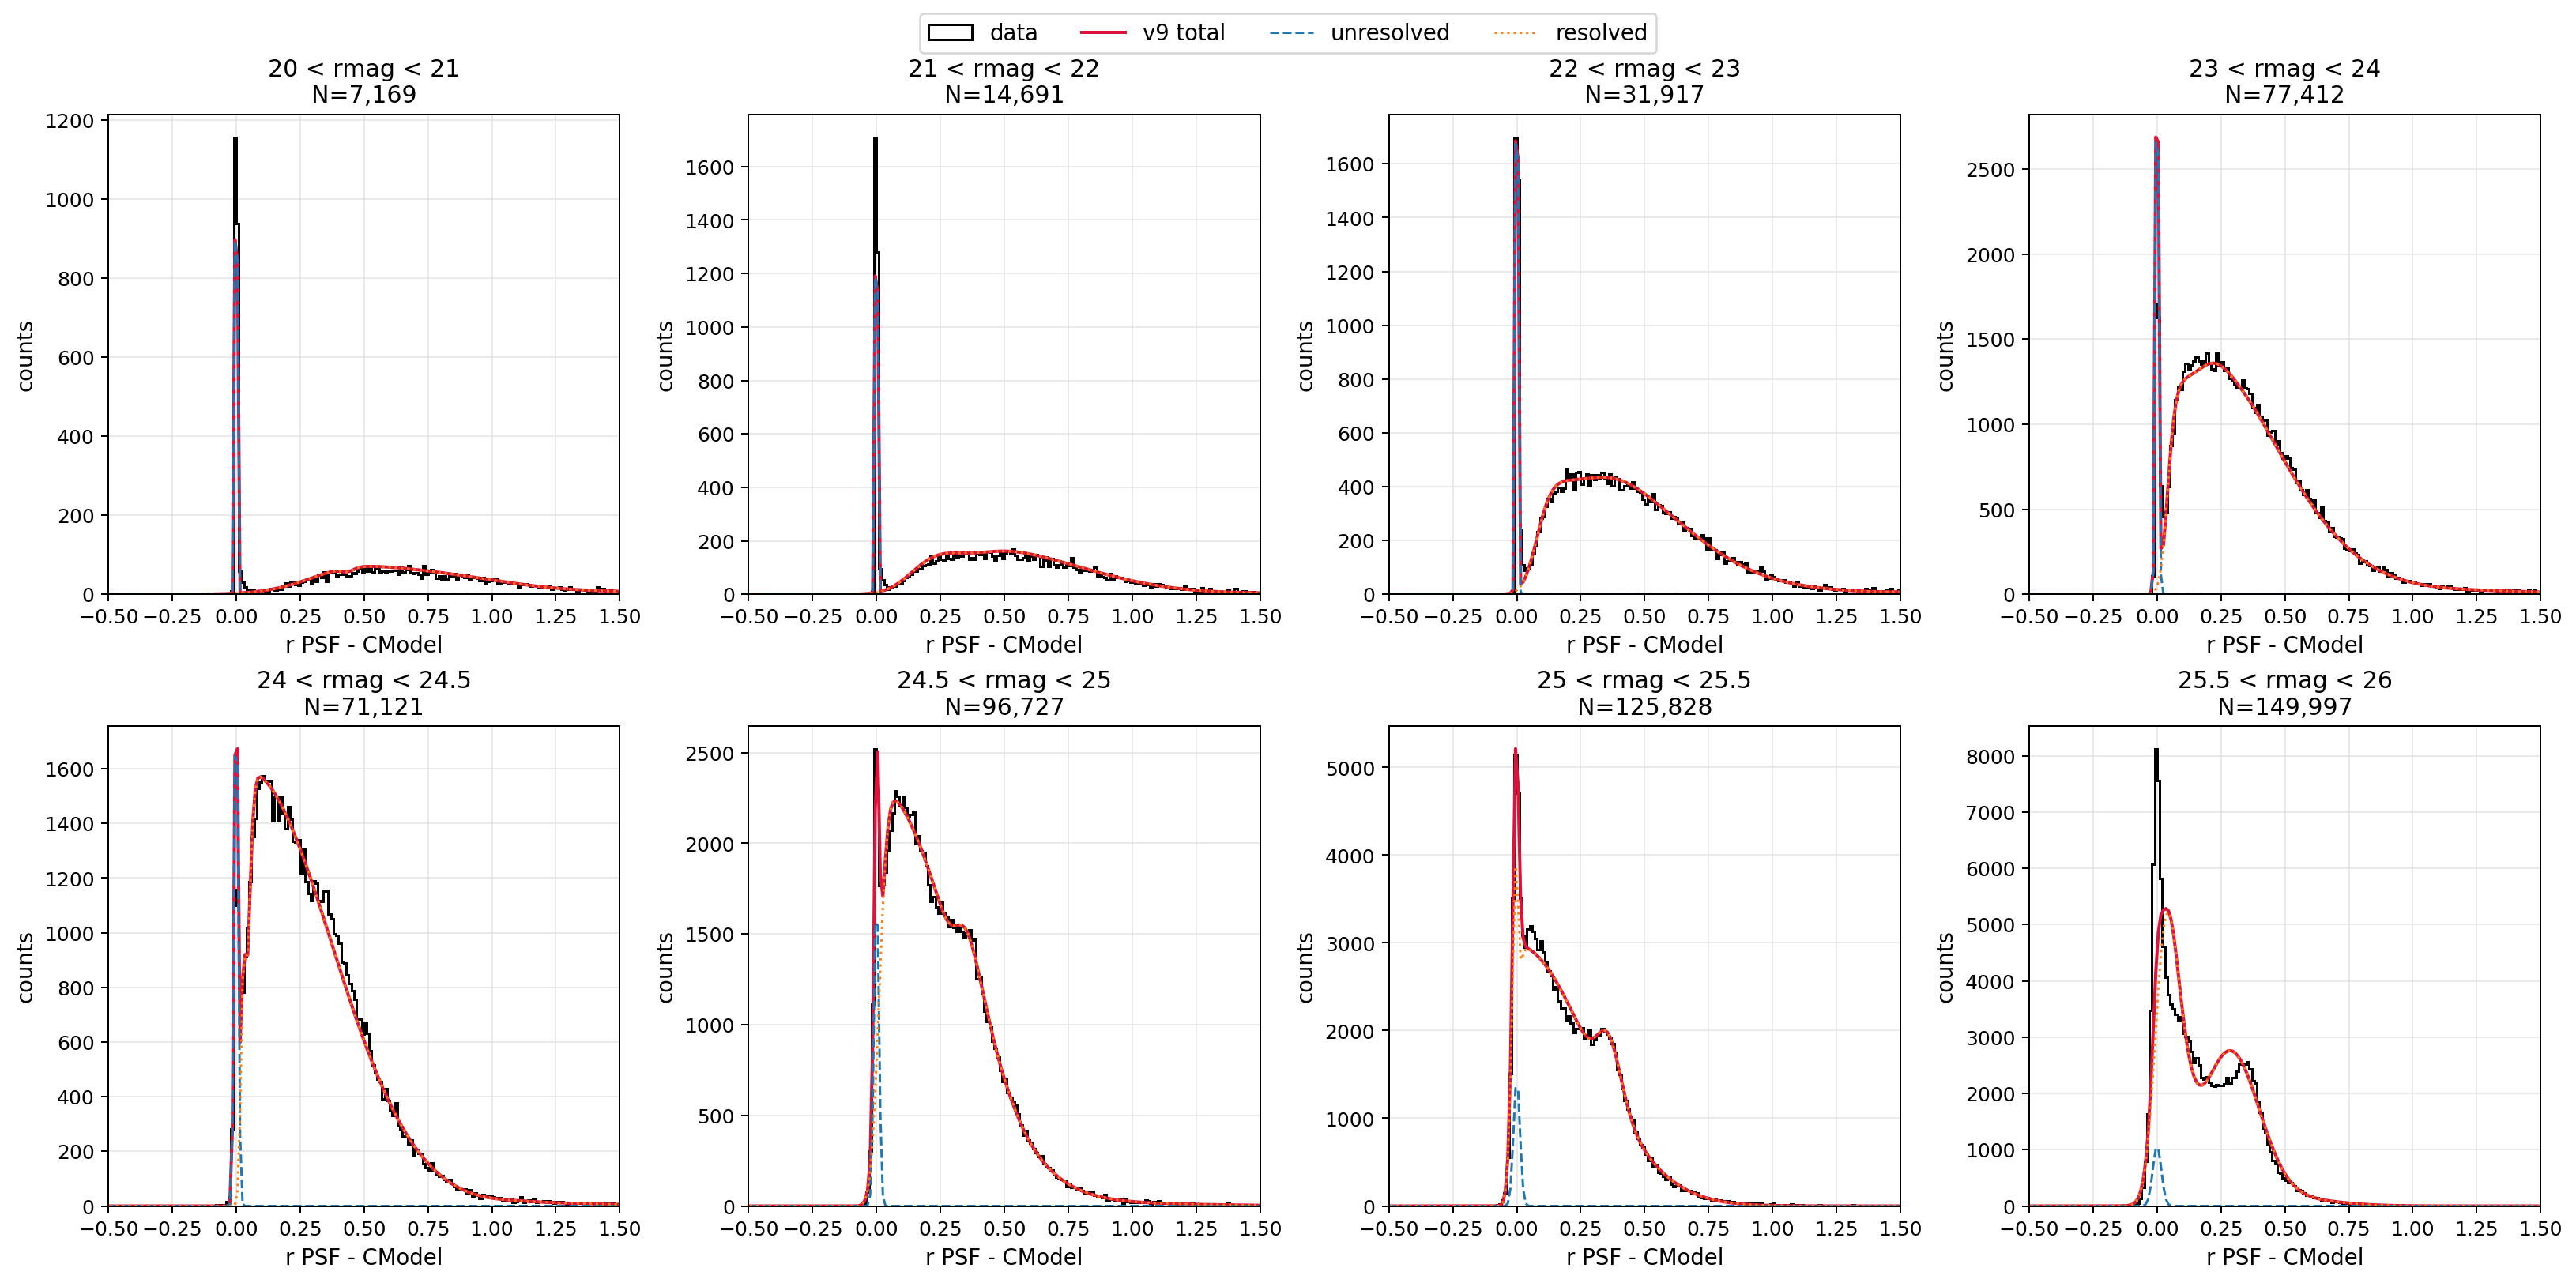
\includegraphics[width=\textwidth,height=0.72\textheight,keepaspectratio]{figures/section2_bayesian_method/fig2_2_cosmos_r_slice_fits_v9fit.png}
  \caption{Observed \(\Delta m\) histograms (black) and fitted mixture models (red) for the
    r-band in each CModel magnitude bin. The unresolved Gaussian component is shown as a blue
    dashed line and the resolved skew-normal components as orange dotted lines.}
  \label{fig:slice_fits}
\end{figure*}

\begin{figure*}
  \centering
  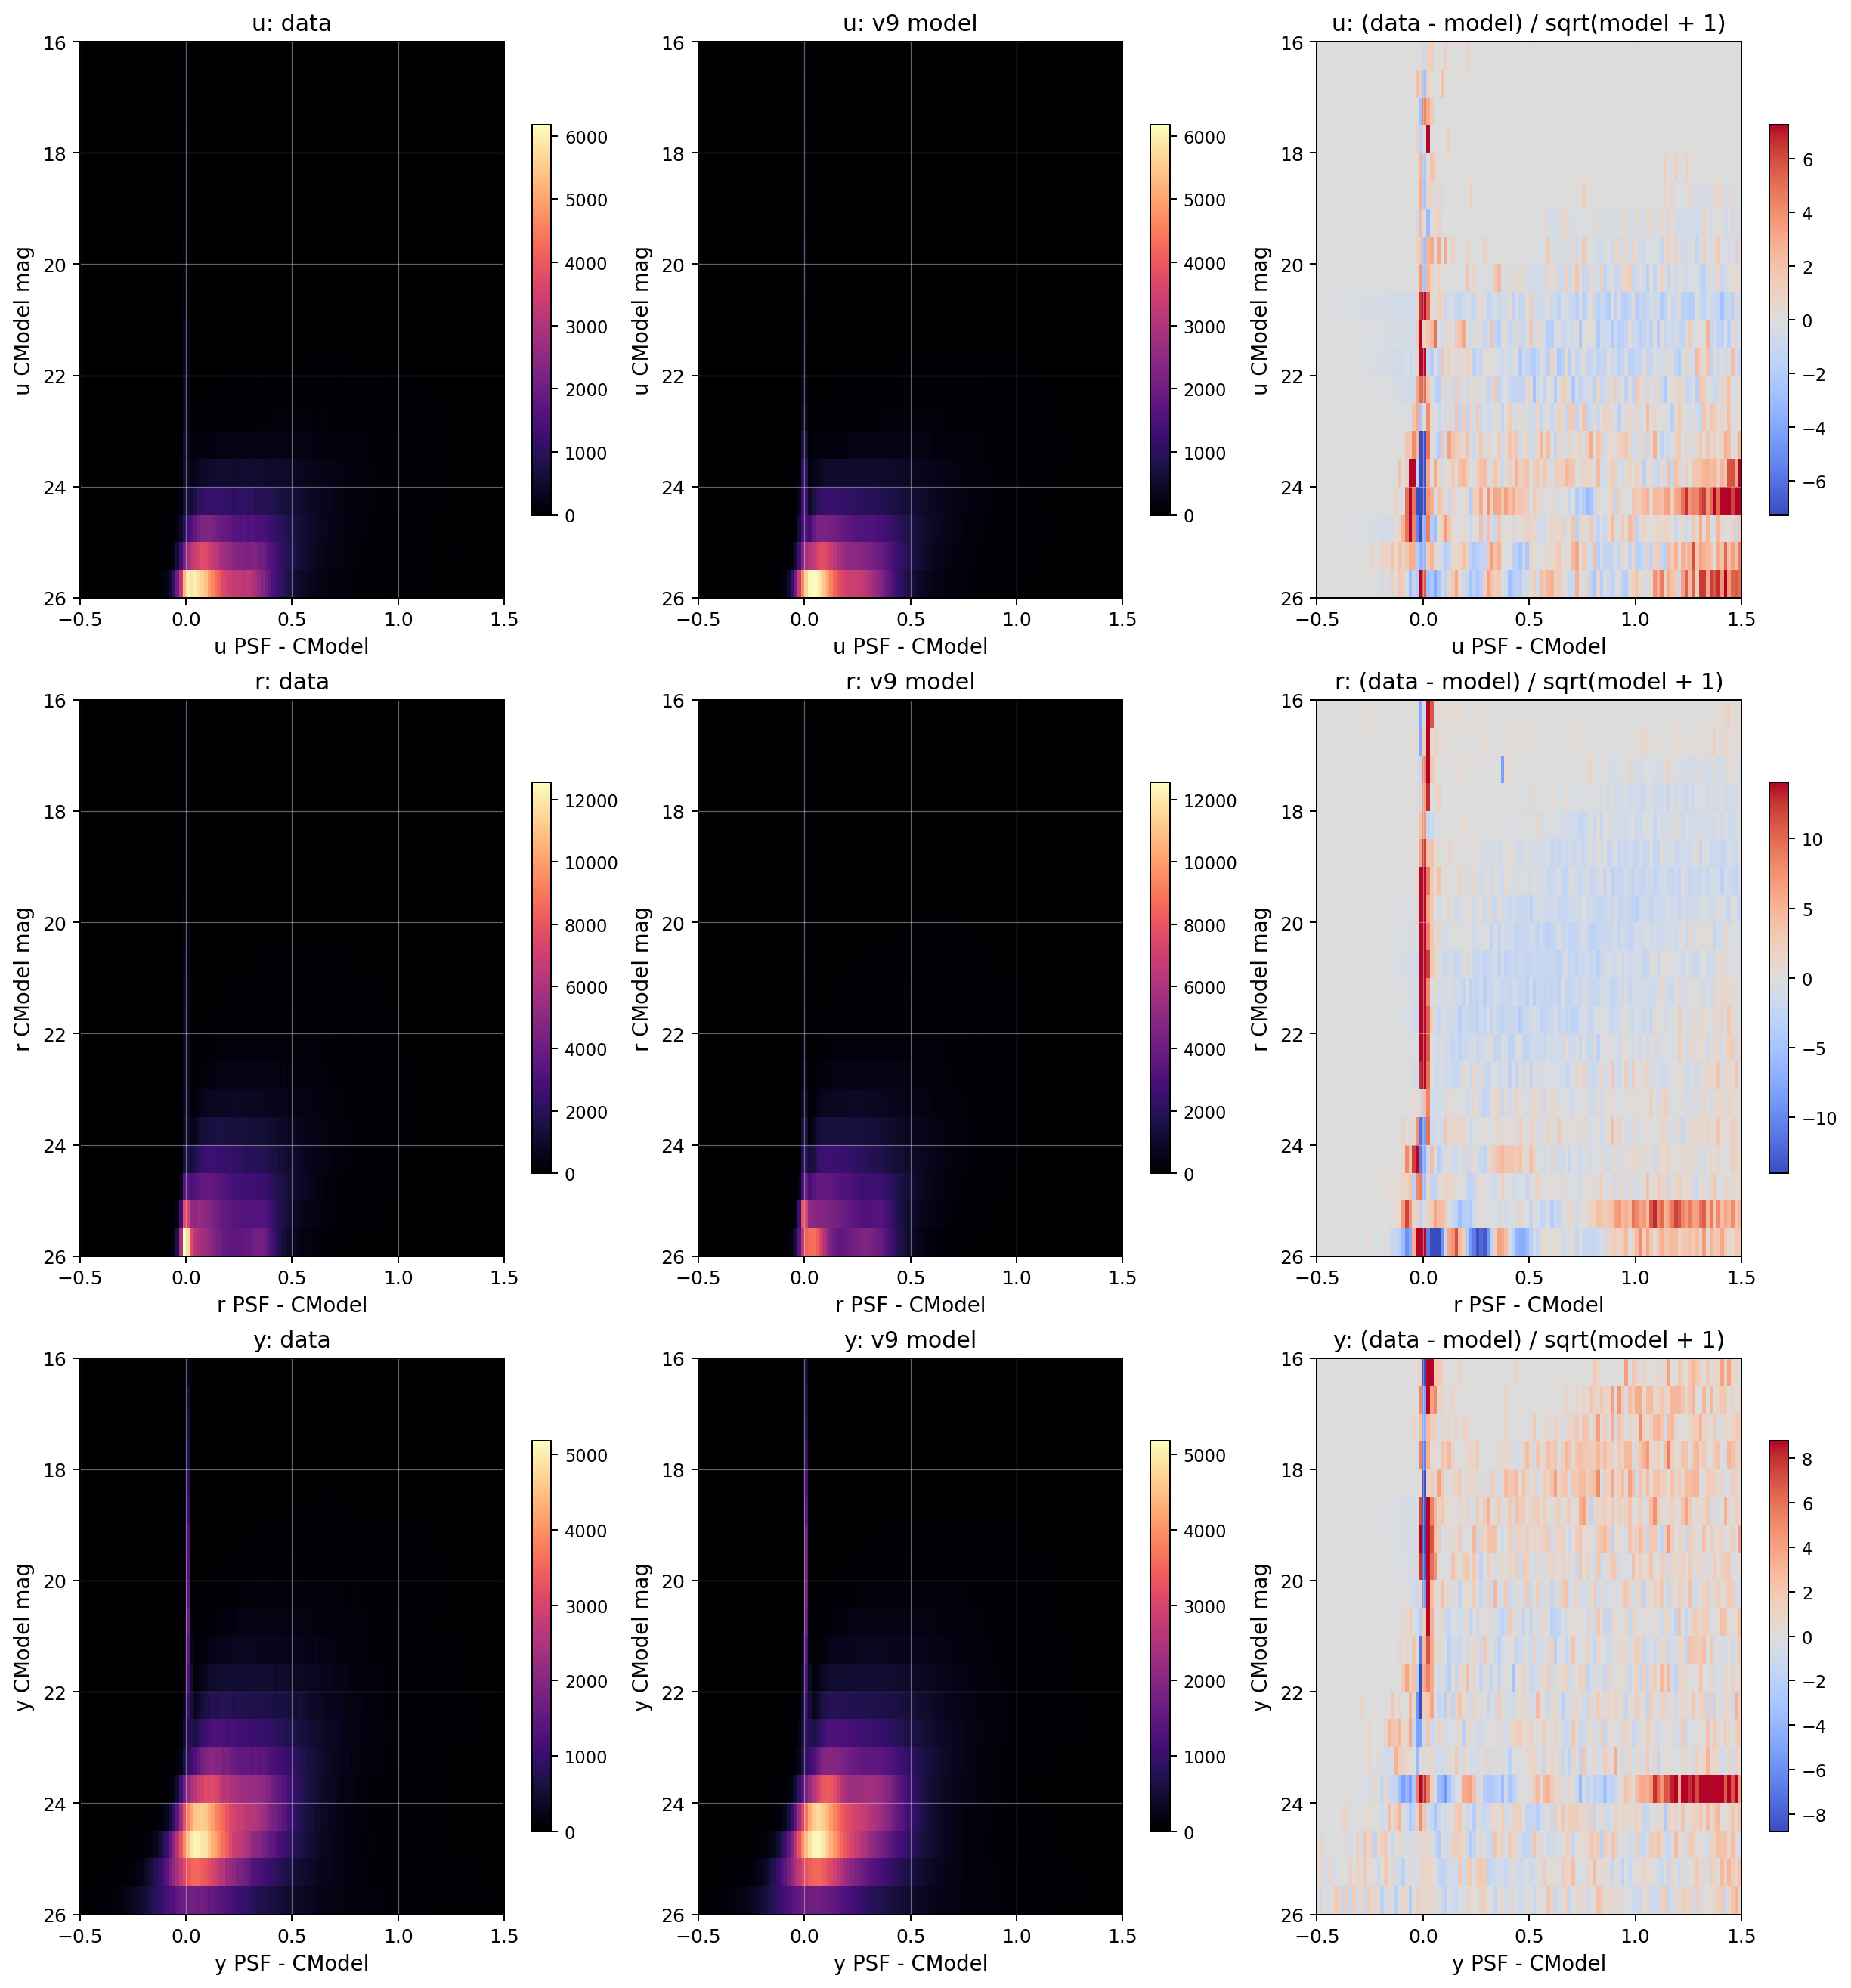
\includegraphics[width=\textwidth,height=0.82\textheight,keepaspectratio]{figures/section2_bayesian_method/fig2_3_cosmos_ury_model2d_residuals_v9fit.png}
  \caption{Two-dimensional comparison of the observed (left), modeled (center), and residual
    (right) source density in the \(\Delta m\) vs.\ \(m_{\mathrm{CModel}}\) plane. The small
    residuals demonstrate that the constrained mixture model provides an adequate description of
    the data across the full magnitude range.}
  \label{fig:model2d_residuals}
\end{figure*}


\subsection{The Performance of the \(\Delta m\) Mixture Model} 

Here we use HST labels to evaluate completeness and contamination for the stellar sample,
and to compare them to mixture model predictions. We focus on the stellar subsample and
the ``transition'' magnitude range: $24 < r < 24.5$: brighter than this limit the population
mixing is much smaller, while fainter than this limit the performance deteriorates rapidly
(especially for the stellar subsample).




 

% Bayes factor: BF(dm) = fG(dm) / fS(dm) 
% pS = fS(dm) / [fS(dm) + fG(dm)]

% pS = 1 / (1 + priorNGS * BF) 

% so 1/pS = 1 + prior * BF = 1 + prior * fG / fS
%    and   pS = 1 / (1 + prior NGS * fG / fS) 




\subsection{The Multi-band Case}

We expect classification to improve with more data but combining the information from different
bands is statistically complex problem... 